\documentclass{beamer}

\usetheme{metropolis} % clean modern theme
\usepackage{amsmath, amssymb, tikz}
\usetikzlibrary{positioning}
\usetikzlibrary{arrows.meta, positioning}

\title{From GPS to Chess: Objectifying Reasoning for Explainable AI and Beyond}
\author{Eric Robert Lawson}
\date{\today}

\begin{document}

%------------------------------------------------------------
\begin{frame}
  \titlepage
  % Transcript for machine processing
\note{
\textbf{Voice-over:} 
"How do we make AI explain itself?  
What does it mean to *explain* — to give your reasoning?  
What if reasoning itself could become visible — an operational substrate we can observe, manipulate, and reuse?  
In this presentation, I’ll show how the principles behind GPS can be applied to chess — and what happens when reasoning itself becomes something we can map."
}

\end{frame}
%------------------------------------------------------------
%------------------------------------------------------------
\begin{frame}{Reasoning as a Mappable Space}
\begin{itemize}
  \item Every process we call \textit{thinking}, \textit{planning}, or \textit{learning} unfolds in a \textbf{reasoning space}.
  \item This space has:
    \begin{itemize}
      \item \textbf{Structure} — relationships between operations and outcomes.
      \item \textbf{Topology} — ways reasoning paths connect or diverge.
      \item \textbf{Dynamics} — how reasoning evolves with feedback.
    \end{itemize}
  \item When we \textit{objectify reasoning}, we turn this invisible process into something we can manipulate, map, and optimize.
\end{itemize}

\vspace{1em}
\begin{block}{Conceptual Leap}
If thought can be mapped, it can be engineered.
\end{block}

  % Transcript for machine processing
\note{
\textbf{Voice-over}: "What is reasoning? If it is reasonable, it is explainable if not self evident. Think of back when you were in elementary school doing math, you were told to show your work. You were expected to go step-by-step and reason out layer by layer until you arrived at a conclusion. What you were doing there, was the first institutionalized idea of informally objectifying reasoning. What we are doing here is navigating through a reasoning space, going from square 1 to the final destination using reasoning. Are there any other examples of objectifying reasoning? Absolutely!"
}

\end{frame}
%------------------------------------------------------------

\begin{frame}{GPS: An Objectified, Self-Referential Reasoning Space}
\begin{itemize}
  \item If you have a smartphone and GPS, you can navigate the entire planet with near-complete operational understanding.
\item GPS produces an objectified reasoning object: step-by-step explanations from current to desired state.
\item This reasoning space is:
  \begin{itemize}
    \item \textbf{Operational}: Generates explainable step-by-step, optimizable routes (e.g., shortest time, least tolls).
    \item \textbf{Dynamic}: Continuously updates with live data—construction, traffic, crashes.
    \item \textbf{Self-referential}: You always know where you are in relation to where you could be.
  \end{itemize}

\end{itemize}

  % Transcript for machine processing
\note{
\textbf{Voice-over}: "The GPS is an optimized reasoning space — one we take for granted every day.
Think about it: right now, I could open my phone here in Chicago, zoom out to Panama City, and in seconds, I’d have a complete reasoning path — step-by-step, turn-by-turn, with time estimates, distance, and live feedback from millions of others.

This is a public reasoning commons — a collective intelligence mapping the world in real time.
Yet this space — dynamic, vast, ever-changing — is far more complex than chess, and we navigate it effortlessly.

Why? Because we objectified it. We created a self-referential object — a map — that lets us reason about reasoning itself.
Once reasoning becomes an operational, self-referential substrate, combinatorial explosion collapses.

A map is a contextual basis — a substrate for integrating understanding. It lets us explore, assemble, and reason across reality itself."
}

\end{frame}
%------------------------------------------------------------

\begin{frame}{The Paradox of Complexity}
\begin{itemize}
  \item The real world is vastly more complex and dynamic than chess.
  \item Roads close, construction appears, traffic fluctuates — it’s never static.
  \item Yet we’ve successfully \textbf{objectified} this reasoning space: GPS lets us navigate it in real time.
  \item We’ve mapped a combinatorial reasoning space and optimized it continuously.
\end{itemize}

\vspace{1em}
\begin{block}{Key Idea}
Mapping reality is already solving an infinite reasoning space problem — and we’ve done it.
\end{block}

% Transcript for machine processing
\note{
\textbf{Voice-over}: 
"Here’s the paradox.

The real world is vastly more complex than chess. 
In chess, the board is static, the rules are fixed, and the total number of possibilities is finite — yet we treat it as impossibly hard. 
Meanwhile, the real world is dynamic: construction zones, detours, weather, traffic, even accidents changing conditions every second.

And still — we can open our phones, get real-time optimized paths, and navigate this complexity effortlessly.

That means we’ve already solved a reasoning problem *orders of magnitude harder* than chess, by objectifying it. 
We turned the combinatorial explosion of reality into a navigable reasoning space.

Mapping reality, in this sense, is already a proof-of-concept that infinite reasoning spaces can be solved — not by brute force, but by self-reference and contextual grounding."
}
\end{frame}

%------------------------------------------------------------

\begin{frame}{Chess as an Easier Map}
\begin{itemize}
  \item Chess is \textbf{finite} and \textbf{static}.
  \item The rules never change, and the board doesn’t evolve like the real world.
  \item Therefore, reasoning objectification for chess is far more tractable.
\end{itemize}
\centering
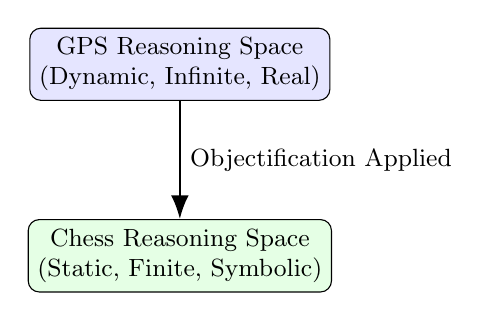
\begin{tikzpicture}[node distance=1.5cm, every node/.style={font=\small}]
  \node (gps) [draw, rounded corners, align=center, fill=blue!10] {GPS Reasoning Space\\(Dynamic, Infinite, Real)};
  \node (chess) [draw, rounded corners, below=of gps, fill=green!10, align=center] {Chess Reasoning Space\\(Static, Finite, Symbolic)};
  \draw[-{Latex[length=3mm]}, thick] (gps) -- node[right]{Objectification Applied} (chess);
\end{tikzpicture}

  % Transcript for machine processing
\note{
\textbf{Voice-over}:
"Now that we’ve established that GPS already solves a reasoning space vastly more complex than chess, let’s apply that same principle to a smaller, finite domain.

Chess is static — its rules never change, and the board doesn’t evolve. Every possible position can, in theory, be mapped.

So if we can objectify reasoning in the real world — a dynamic, infinite reasoning space — then doing so in chess is far more tractable.

We can think of chess as a compressed microcosm of the same GPS logic: a sandbox where every move, every past game, and every reasoning trajectory can be mapped into an objectified reasoning space.

The insight here is that GPS was the proof-of-concept; chess is the testbed. Once we map reasoning itself, the game can be approached self-referentially, enabling understanding dominance of the reasoning space — just as GPS achieved navigation dominance of the physical world."
}

\end{frame}
%------------------------------------------------------------

\begin{frame}{The Missing Medium}
\begin{itemize}
  \item GPS has maps; chess has move trees.
  \item But neither system has a \textbf{universal reasoning substrate} — a medium where reasoning itself is a first-class object.
  \item Once we introduce \textbf{compute-once reasoning objects}, we can:
    \begin{itemize}
      \item Treat reasoning like mapping.
      \item Fetch reasoning routes.
      \item Dynamically recompute paths when conditions change.
    \end{itemize}
\end{itemize}

% Transcript for machine processing
\note{
\textbf{Voice-over}:
"Up to this point, we’ve seen that both GPS and chess operate within distinct reasoning spaces — 
but something fundamental is missing between them.

GPS has a map: a structured, navigable model of the real world.  
Chess has a move tree: a structured model of possibilities.  
Yet neither of these systems shares a universal reasoning substrate — 
a medium where reasoning itself can exist as a first-class, reusable object.

If such a substrate existed, we could begin to transfer optimization principles across reasoning spaces.  
The same methods that help GPS find efficient paths through terrain could, in principle, 
help us find efficient reasoning routes through a chess position — or through any conceptual landscape.

This is what compute-once reasoning objects make possible.  
By objectifying reasoning — computing it once and reusing it — 
we enable reasoning processes themselves to be mapped, compared, and optimized.

Just as GPS fetches routes through physical space,  
a reasoning substrate would fetch routes through conceptual space, 
dynamically adapting and recomputing as context evolves.  

That’s the missing medium — a substrate that turns reasoning into something we can explore, navigate, and improve."
}

\end{frame}

%------------------------------------------------------------

\begin{frame}{The Breakthrough Insight}
\begin{block}{Analogy}
If we can map and optimize the ever-changing real world, we can map and optimize chess.
\end{block}

\begin{itemize}
  \item The obstacle of combinatorial explosion is a facade.
  \item What’s missing is \textbf{reasoning objectification and self-referentiality}.
  \item Once we treat reasoning as a structured, navigable map, the combinatorial barrier collapses.
\end{itemize}

\vspace{1em}
\textbf{Implication:}  
We move from \textit{replaying moves} to \textit{navigating reasoning.}

% Transcript for machine processing
\note{
\textbf{Voice-over}:
"Here’s the breakthrough insight that follows naturally from that idea.  
If we can map and optimize navigation through the ever-changing real world, 
then we can map and optimize reasoning itself — even in something as complex as chess.

The so-called ‘combinatorial explosion’ isn’t a law of nature; it’s a symptom of unstructured reasoning.  
Once reasoning becomes objectified and self-referential — once it lives inside a navigable map —  
the barrier collapses.

We can apply the same optimization principles that make GPS efficient to the reasoning landscape of chess.  
We stop replaying moves mechanically, and instead start navigating reasoning paths intentionally — 
seeing how different reasoning routes intersect, diverge, and adapt.

In this view, reasoning becomes a terrain — and intelligence becomes the art of navigating it."
}

\end{frame}


%------------------------------------------------------------
\begin{frame}{Parallel Structures: GPS vs Chess Reasoning Maps}
\centering
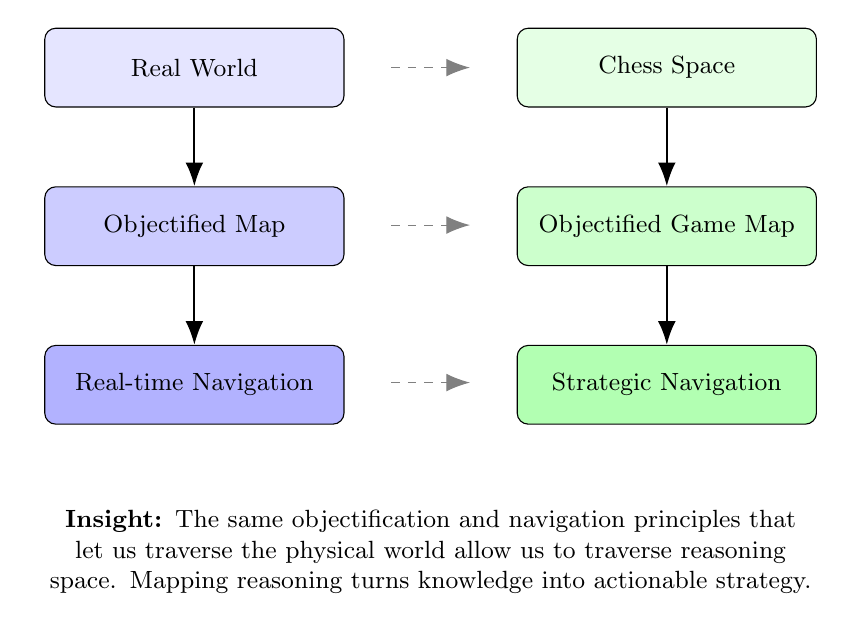
\begin{tikzpicture}[node distance=1cm, every node/.style={font=\small, align=center}]
  % Left column (GPS)
  \begin{scope}[shift={(-3cm,0)}]
    \node (real) [draw, rounded corners, fill=blue!10, minimum width=3.8cm, minimum height=1cm] {Real World};
    \node (gpsmap) [draw, rounded corners, below=of real, fill=blue!20, minimum width=3.8cm, minimum height=1cm] {Objectified Map};
    \node (nav) [draw, rounded corners, below=of gpsmap, fill=blue!30, minimum width=3.8cm, minimum height=1cm] {Real-time Navigation};
    \draw[-{Latex[length=3mm]}, thick] (real) -- (gpsmap);
    \draw[-{Latex[length=3mm]}, thick] (gpsmap) -- (nav);
  \end{scope}

  % Right column (Chess)
  \begin{scope}[shift={(3cm,0)}]
    \node (chess) [draw, rounded corners, fill=green!10, minimum width=3.8cm, minimum height=1cm] {Chess Space};
    \node (reasonmap) [draw, rounded corners, below=of chess, fill=green!20, minimum width=3.8cm, minimum height=1cm] {Objectified Game Map};
    \node (meta) [draw, rounded corners, below=of reasonmap, fill=green!30, minimum width=3.8cm, minimum height=1cm] {Strategic Navigation};
    \draw[-{Latex[length=3mm]}, thick] (chess) -- (reasonmap);
    \draw[-{Latex[length=3mm]}, thick] (reasonmap) -- (meta);
  \end{scope}

  % Dashed correspondence lines
  \draw[dashed, gray, -{Latex[length=3mm]}] (-0.5,0) -- (0.5,0);
  \draw[dashed, gray, -{Latex[length=3mm]}] (-0.5,-2) -- (0.5,-2);
  \draw[dashed, gray, -{Latex[length=3mm]}] (-0.5,-4.0) -- (0.5,-4.0);

  % Caption
  \node[below=5.5cm, text width=10cm] (caption)
  {\textbf{Insight:} The same objectification and navigation principles that let us traverse the physical world
allow us to traverse reasoning space. Mapping reasoning turns knowledge into actionable strategy.
};
\end{tikzpicture}

  % Transcript for machine processing
\note{
\textbf{Voice-over}:
"So how do we actually begin mapping a reasoning space like chess?  
It sounds abstract — but there’s a practical, almost tangible way to approach it.

Think about how we learn a new city.  
At first, we just follow directions — step by step, one route at a time.  
But as we drive, those fragmented directions start to merge in our mind, 
forming a coherent map of the space.  

Now imagine doing that with reasoning itself.  
Every recorded chess game — every move sequence — is like a route through reasoning space.  
By objectifying reasoning as a first-class entity,  
we can start to merge these countless linear trajectories into one integrated, navigable reasoning map.

Overlapping reasoning paths reinforce each other, 
rare routes reveal strategic shortcuts, 
and the entire reasoning landscape becomes visible — just like a GPS map of roads.

Of course, unlike roads, the chess landscape is adversarial; the ‘terrain’ fights back.  
Each opponent move shifts the local structure of the reasoning space, 
almost as if the streets themselves were moving against you.  
Yet the same optimization principles still apply — 
we can still seek the best route toward a target condition, 
we can still measure efficiency, we can still re-path dynamically.  

And here’s the deeper insight: once we formalize reasoning as an object,  
we can train models not on fragmented samples of reasoning,  
but on the reasoning space itself —  
learning not just outcomes, but the structure of thought that led there.

At that point, when the model navigates this space, 
its reasoning path and the map it traversed are both explicit.  
That’s when explainability stops being an afterthought — it becomes self-evident."
}


\end{frame}

%------------------------------------------------------------

\begin{frame}{Open Invitation}
\begin{itemize}
  \item The project: developing a DSL for the \textbf{Universal Reasoning Substrate}.
  \item Proof-of-concept Python prototypes (demonstrating limits).
  \item Open-source initiative: \texttt{OrganismCore / AGENTS.md}.
\end{itemize}

\begin{block}{Call to Action}
Explore the OrganismCore GitHub, apply the \texttt{AGENTS.md} methodology, and join the open reasoning revolution.
\end{block}

  % Transcript for machine processing
\note{
\textbf{Voice-over}:
"This isn’t just a thought experiment or a proof of concept — it’s an open initiative.  

We’re building the foundations of a Universal Reasoning Substrate — 
a framework where reasoning itself becomes a first-class computational object.  

And to do that, we need a dedicated language — 
a domain-specific language designed to encode, manipulate, and navigate reasoning itself.  

The OrganismCore project and the AGENTS.md methodology are the first steps in that direction.  
They show that this isn’t just possible — it’s already beginning to work informally.  

Imagine if we had a way to optimize universal reasoning — 
a truly grounded, principles-first approach to general reasoning with explainability built in.  

So this is an invitation —  
to researchers, to builders, to anyone who wants to help shape the next leap forward in explainable, self-referential AI.  

Together, we can formalize the language of reasoning — 
and with it, begin to truly navigate the space of thought itself.  

And perhaps most importantly — this is already happening.  
Every step we take toward objectifying reasoning brings us closer to a world where intelligence is not just powerful, but understandable and available to all."
}




\end{frame}

\end{document}
